\documentclass{entcs} 
\usepackage{entcsmacro}
\usepackage{graphicx}
\usepackage{code}

\newcommand{\cut}[1]{}

\newcommand{\appref}[1]{Appendix~\ref{#1}}
\newcommand{\secref}[1]{Section~\ref{#1}}
\newcommand{\tblref}[1]{Table~\ref{#1}}
\newcommand{\figref}[1]{Figure~\ref{#1}}
\newcommand{\listingref}[1]{Listing~\ref{#1}}
%\newcommand{\pref}[1]{{page~\pageref{#1}}}

\newcommand{\eg}{{\em e.g.}}
\newcommand{\cf}{{\em cf.}}
\newcommand{\ie}{{\em i.e.}}
\newcommand{\etc}{{\em etc.\/}}
\newcommand{\naive}{na\"{\i}ve}
\newcommand{\role}{r\^{o}le}
\newcommand{\forte}{{fort\'{e}\/}}
\newcommand{\appr}{\~{}}

\newcommand{\bftt}[1]{{\ttfamily\bfseries{}#1}}
\newcommand{\kw}[1]{\bftt {#1}}
\newcommand{\Pthen}{\kw{Pthen}}
\newcommand{\pads}{\textsc{pads}}
\newcommand{\padsl}{\textsc{padsl}}
\newcommand{\padst}{\textsc{pads/t}}
\newcommand{\datatype}{\textsc{PADS/T}}
%\newcommand{\datatype}{\textsc{DataType}}
\newcommand{\C}{\textsc{C}}
\newcommand{\perl}{\textsc{Perl}}
\newcommand{\ml}{\textsc{ml}}
\newcommand{\sml}{\textsc{sml}}
\newcommand{\smlnj}{\textsc{sml/nj}}
\newcommand{\java}{\textsc{java}}
\newcommand{\ddl}{\textsc{ddl}}
\newcommand{\xml}{\textsc{xml}}
\newcommand{\datascript}{\textsc{DataScript}}
\newcommand{\packettypes}{\textsc{PacketTypes}}
\newcommand{\erlang}{\textsc{Erlang}}

\newcommand{\Core}{Ad hoc}
\newcommand{\core}{ad hoc}
\newcommand{\pvalue}{\core{} value}
\newcommand{\ppat}{\core{} pattern}
\newcommand{\ptype}{\core{} type}

\newcommand{\padsc}{\textsc{pads}/\C{}}
\newcommand{\padsml}{\textsc{pads}/\ml{}}

\newcommand{\dibbler}{Sirius}
\newcommand{\ningaui}{Altair}
\newcommand{\darkstar}{Regulus}

\newcommand{\pdgood}{{\tt G}}
\newcommand{\pdbad}{{\tt B}}
\newcommand{\pdnest}{{\tt N}}
\newcommand{\pdsem}{{\tt S}}
\newcommand{\ptypes}{T}
\newcommand{\patreadpd}[2]{{\tt #1<<#2>>}}
\newcommand{\btm}{\cd{BOT}}


\newcommand{\lsem}{{[\![}}
\newcommand{\rsem}{{]\!]}}


\newcommand{\figHeight}[4]{\begin{figure}[tb]
	\centerline{
	            \epsfig{file=#1,height=#4}}
	\caption{#2}
	\label{#3}
	\end{figure}}

%% Environment for typesetting BNF grammars. Uses display math mode.
\newenvironment{bnf}
     {%% local command definitions:
        %% BNF definition symbol
      \def\->{\rightarrow}
%%      \def\::={{::=} &}
      \def\::={\bnfdef &}
      \def\|{\bnfalt}
      \newcommand{\name}[1]{\text{##1}}
        %% non-terminal
      \newcommand{\nont}[1]{{##1}}
      \newcommand{\meta}[1]{& ##1 &}
      \newcommand{\descr}[1]{& \text{// ##1}}
      \newcommand{\opt}[1]{ [##1] }
      \newcommand{\opnon}[1]{\opt{\nont{##1}}}
      \newcommand{\none}{\epsilon}
      \newcommand{\nwln}{\\ &&&}
      \newcommand{\nlalt}{\\ && \| &}
      \[\begin{array}{lrlll}
     }
     {\end{array}\]}

\newcommand{\mcd}[1]{\mathtt{#1}}
\newcommand{\ppair}[3]{#1{:}#2 \mathrel{**} #3}
\newcommand{\parray}[3]{#1\;\mcd{Parray}(#2,#3)}
\newcommand{\pset}[3]{\{#1{:}#2\,|\,#3\}}
\newcommand{\pstream}[1]{#1\;\mcd{stream}}
\newcommand{\precord}[1]{\{\{#1\}\}}


% A couple of exemplary definitions:
\def\lastname{Fernandez, Fisher, Mandelbaum and Walker}
\begin{document}
\begin{frontmatter}
  \title{\datatype{}: Language Support for Processing Ad Hoc Data Sources} 
  \author{Maria Fernandez,
    Kathleen Fisher\thanksref{attemail}}
  \address{AT\&T\\ 
    Florham Park,NJ USA} 
  \author{Yitzhak Mandelbaum,
    David Walker\thanksref{premail}}
  \address{Department of Computer Science\\ 
    Princeton University\\
    Princeton,NJ USA} 
  \thanks[attemail]{Email:\texttt{\normalshape
        mff,kfisher@research.att.com}}
  \thanks[premail]{Email:\texttt{\normalshape
        yitzhakm,dpw {\it at} cs {\it dot} princeton {\it dot} edu}}
\begin{abstract} 
  Insert abstract here.
\end{abstract}
\begin{keyword}
  Please list keywords from your paper here, separated by commas.
\end{keyword}
\end{frontmatter}

\section{Introduction}
\label{intro}

An {\em ad hoc data format} is any nonstandard data format for which
parsing, querying, analysis or transformation tools are not readily
available.  \xml{} is not an ad hoc data format --- there are hundreds
of tools for reading, querying, and transforming \xml{}.  However,
computer programmers, financial analysts, computational biologists,
chemists and physicists, healthcare and airline information systems,
corporate IT professionals and others deal with deal ad hoc data in a
myriad of complex formats on a daily basis.  This data is often
unpredictable, poorly documented, and filled with errors, making it
extremely difficult to deal with.  Often, before anything can be done
with ad hoc data one must clense it of as many errors as possible,
normalize its shape and transform it into a standardized format.  Once
in a standardized format, the data can be directly loaded into a
database or manipulated by standard, widely available tools.

% The goal of this paper is to describe a new language for efficient and
% reliable computing with ad hoc data.  More specifically, we describe a
% high-level programming language, \datatype{}, that comes with
% intrinsic support for processing ad hoc data.  Our programming
% language will use the rich data descriptions both as directives for
% parsing ad hoc data sources and as types for describing
% representations of ad hoc data within the programming environment.  In
% addition, a critical facet of our language will be its support for
% {\em error-aware computing}.  Our error-aware infrastructure will
% allow programmers to conveniently verify correctness of data relative
% to a description or alternatively detect data errors and handle them
% in domain-specific ways.  Finally, we will be sure our language design
% is founded on strong programming language principles by studying its
% type system and metatheory extensively.

There are vast amounts of useful data stored in traditional databases
and \xml{} formats, but there is just as much in ad hoc formats.
\figref{figure:data-sources} provides some information on ad hoc data
formats from the networking and telecommunications domain at AT\&T and
ad hoc data formats used by computational biologists at Princeton.
They include ASCII, binary, and Cobol data formats, with both fixed
and variable-width records arraged in linear sequences or in tree- or
DAG-shaped hierarchies.  The data sources range in size from
relatively small files up to network applications, such as web server
logs, which can be produced at a rate of 12GB per week, to Netflow
applications, which can be produced at over one GB per second.  Common
errors include undocumented data, corrupted data, missing data, and
multiple missing-value representations.

We hope that these examples give the reader a beginning sense of the
nature and pervasiveness of ad hoc data sources.  However, we cannot
emphasize enough just how pervasive ad hoc data is and to what degree
it infiltrates computer systems, businesses, government, and
scientific research.  Remember, just about any program that spits out
useful information in a format other than \xml{}, \textsc{html},
\textsc{jpeg}, \textsc{mpeg} or a few others is generating ad hoc
data.  Hence, most programmers deal with ad hoc data on a individual
basis regularly.  When it comes to ad hoc data on a grand scale,
perhaps the most daunting challenge will come from the national
health-care system.  Recently, Newt Gingrich and Hilary Clinton have
jointly proposed we consolidate and integrate our national healthcare
records in the next 10 years.  Such a massive project will undoubtedly
require technical solutions at many levels.  At the lowest levels, we
will need a reliable software to collect and transfer health care data
from legacy systems into modern formats.  The \datatype{} system we
propose will be an invaluable aid in the development of this software.

\begin{figure*}
\begin{center}
\begin{tabular}{@{}|l|l|l|l|}
\hline
Name: Use                           & Representation    
%& Size
           & Common Errors \\ \hline\hline
Web server logs (CLF):                & Fixed-column      
%& $\leq$12GB/week 
& Race conditions on log entry\\ 
Measuring web workloads               & ASCII records     
%&                             
& Unexpected values\\ \hline
AT\&T provisioning data (\dibbler{}): & Variable-width    
%& 2.2GB/week 
& Unexpected values \\ 
Monitoring service activation         & ASCII records     
%&            
& Corrupted data feeds \\ \hline
Call detail:                   & Fixed-width       
%&\appr{}7GB/day 
&  Undocumented data\\
Fraud detection 
                                      & binary records  
%& 
& \\ \hline 
AT\&T billing data (\ningaui{}):      & Cobol  
%& \appr{}4000 files/day, 
& Unexpected values\\ 
Monitoring billing process   &                             
%& 250-300GB/day    
& Corrupted data feeds \\ \hline
IP backbone data (\darkstar{})  & ASCII  
%& $\ge$ 15 sources  
& Multiple missing-value rep's \\
Network Monitoring:  &        
%& \appr{}15 GB/day              
& Undocumented data \\ \hline
Netflow                               & Data-dependent      
%& $\ge$1Gigabit/second  
& Missed packets\\ 
Network Monitoring:        & number of   
%&                       
& \\
                                      & fixed-width 
%&
& \\
                                      & binary records 
%&
& \\ \hline
Gene Ontology data:        & Variable-width ASCII records 
%& ? 
&  \\
Gene-gene correlations in Magic & in DAG-shaped hiearchy 
%&  
& \\
database &
%& 
& \\\hline
Newick data                          & Fixed-width ASCII record 
%& ? 
& Manual entry errors \\
Immune system response simulation & in tree-shaped hierarchy 
%& 
& \\
\hline
\end{tabular}
\caption{Selected ad hoc data sources.}
\label{figure:data-sources}
\end{center}
\end{figure*}

Processing all this ad hoc data is challenging for a variety of
reasons.  First, ad hoc data typically arrives ``as is'': the analyst
or system that receives it can only say ``thank you,'' not request a
more convenient format.  Second, documentation for the format may not
exist at all, or it may be out of date.  A common phenomenon is for a
field in a data source to fall into disuse.  After a while, a new
piece of information becomes interesting, but compatibility issues
prevent data suppliers from modifying the shape of their data, so
instead they hijack the unused field, often failing to update the
documentation in the process.

Third, such data frequently contain errors for a variety of reasons:
malfunctioning equipment, race conditions on log entry~\cite{wpp},
non-standard values to indicate ``no data available,'' human error in
entering data, unexpected data values, \etc{} The appropriate response
to such errors depends on the application.  Some applications require
the data to be error free: if an error is detected, processing needs
to stop immediately and a human must be alerted.  Other applications
can repair the data, while still others either set data aside for a
human user to investigate or simply discard the erroneous or
unexpected values altogether.  For some applications, errors in the
data can be the most interesting part because they can signal where
two systems are failing to communicate.

A fourth challenge is that ad hoc data sources can be high volume:
AT\&T's call-detail stream contains roughly 300~million calls per day
requiring approximately 7GBs of storage space. Although this data is
eventually archived in a database, analysts mine it profitably before
such archiving~\cite{kdd98,kdd99}. More challenging, the \ningaui{}
project at AT\&T accumulates billing data at a rate of 250-300GB/day,
with occasional spurts of 750GBs/day. Netflow data arrives from Cisco
routers at rates over a gigabyte per second~\cite{gigascope}! Such
volumes mean it must be possible to process the data without loading
it all into memory at once.

A final challenge is that ad hoc data often needs to be translated
into a new, more useful or more standard format before anything can be
done with it.  Intuitively, this transformation can be done in three
stages.  First, one must generate a parser for the ad hoc format to
read it into a program.  Second, one must engineer the transformation
itself by filtering unwanted parts, normalizing representations, and
detecting and correcting or deleting erroneous data.  Third,
transformed data must be printed in the new format that can be
processed by standards tools.

Examples:Darkstar, Gigascope, Richard at Princeton, Olga/Magic.

Today, people tend to use \C{} or \perl{} for this task.
Unfortunately, writing parsers, transformations and printers this way
is tedious and error-prone, complicated by the lack of documentation,
convoluted encodings designed to save space, the need to produce
efficient code, and the need to handle errors robustly to avoid
corrupting down-stream data.  Moreover, the parser writers' hard-won
understanding of the data ends up embedded in parsing code, making
long-term maintenance difficult for the original writers and sharing
the knowledge with others nearly impossible.

Solution: Data description Language + transform language
Combine data description language with a transform language.
\pads{} is bound to C. However, functional programming languages are
better suited to the task of data tranformation. We therefore propose
a new language, \datatype{}, that combines a data description language
based in the style of ML types (and datatypes) with a functional data
transformation language. 

Our contributions are twofold. First, we propose an ML-style syntax
for the \pads{} data description language, based on type definitions
and {\em(polymorphic coming soon?)} parameterized recursive datatypes
(support for recursive datatypes is new to the \pads{} language, based
on recent results in our other work). This new syntax has a number of
advantages. It is more concise than the C-style encoding and more
naturally suited to describing recursive datatypes. Most importantly,
the new syntax is much more appropriate for transformation language
proposed below, which is based heavily on pattern-matching and data
constructors.

Our second contribution is the data transformation language itself.
{\em \pads{} is not a programming language.}  It merely generates
libraries that can be used by \C{} programmers.  \C{} is a very
low-level language that makes transforming ad hoc data awkward,
cumbersome and potentially error-prone.  More importantly, it provides
no intrinsic support for dealing with the errors that appear in ad hoc
data.  In addition, \C's type system and operational model provide no
support for checking the rich invariants found in ad hoc data either
at run time or at compile time.  In contrast, \datatype{} is a
high-level language with an elegant and convenient syntax for
data-driven programming, intrinsic support for handling errors and
intrinsic mechanisms for checking data invariants at run time {\em
  coming soon: and a sophisticated type system for enforcing data
  invariants at compile time}. 

At its core, \datatype{} is a functional language with standard
features such as pattern matching and higher-order functions, which we
view as critical to supporting data-driven transforms. In addition,
\datatype{} will allow programmers to enforce semantic constraints on
data by using \datatype{} descriptions as a special form runtime
contracts. The basic values of the language will be pairs of data
items and their corresponding meta-data. For each data item, the meta
data will include, among other things, descriptions of the error
content of the data item. Through the type system, the language will
ensure that data and associated meta data are kept in sync. This
property (which we call ``error-aware computing'') enables three
critical language features.
\begin{enumerate}
\item Safe, error-transparent transformations
\item Flexible, programmatic repair of faulty records - analyst can
  choose when in the processing stream to address errors, rather than
  being forced to drop all faulty records at the beginning of the process.
\item Error querying - analyst can extract detailed picture of data
  error profile.
\end{enumerate}

In the next section, we will describe, in detail, the \pads{} approach
to data and meta data (inherited by \datatype{}), the \datatype{}
syntax for data description, and illustrative examples. Next, in
section~\ref{sec:data-transformation} we will elaborate on \datatype{}'s support for
data transformation, including design, syntax, brief overview of the semantics
and some examples. Section~\ref{sec:implementation-techniques} will discuss our proposed
implementation techiniques, and section~\ref{sec:related-work}, the
related work. A discussion of conclusions and future work is concluded
in section~\ref{sec:conclusion}.

\section{Describing Data in \datatype{}}
\label{sec:data-description}

\subsection{The \pads{} Weltanshauung}

\begin{figure}[tp]
  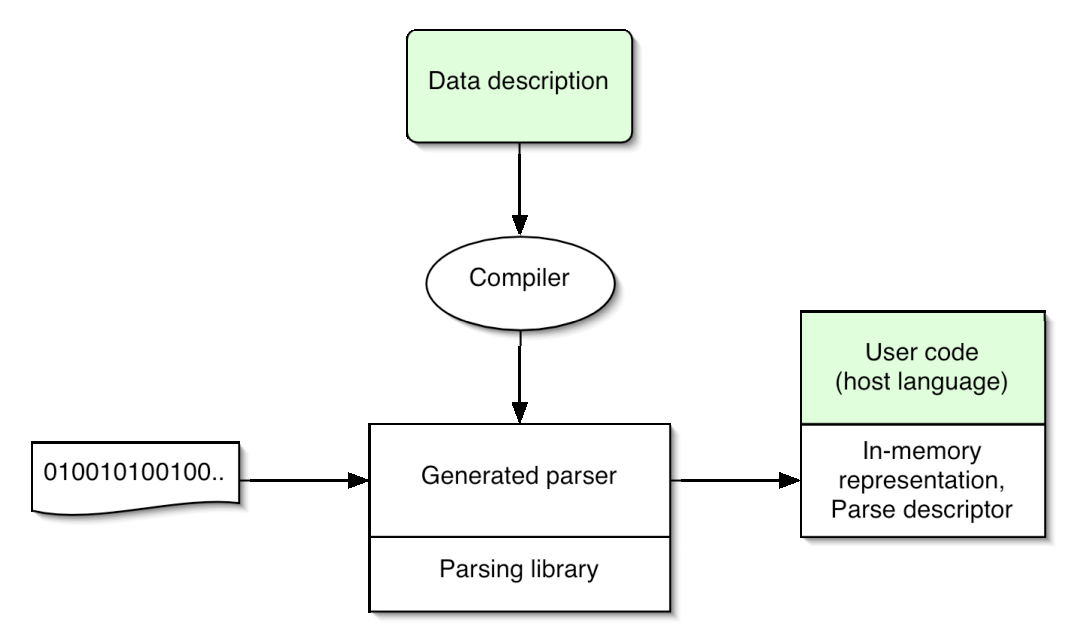
\includegraphics[height=3in,width=5in]{architecture.eps}
%  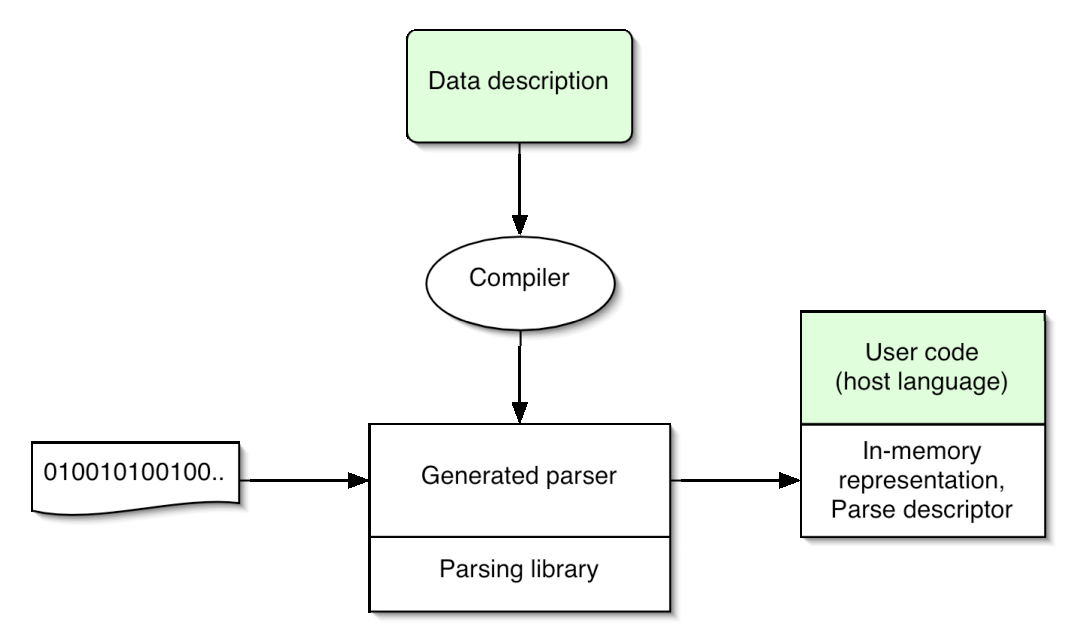
\includegraphics{architecture.eps}
\label{fig:pads-arch}
\caption{The \pads{} Architecture}
\end{figure}

The data description primitives of the \pads{} language are types.
However, more than describing data alone, these types describe a
transformation from data in an external format to data in an internal
format.  Yet, in \pads{}, data does not live alone. A critical benefit
of the parsing is the meta-data gained during the transformation
process.  Therefore, the result of a parse is a pair consisting of a
canonical in-memory representation of the data and meta-data for the
parse.  We refer to the meta-data as the {\em parse descriptor}. The
parse descriptor may hold a variety of bits of information including
the position of the data in the file and a characterization of the
possible errors in the data.  There are several different sorts of
errors that may arise.  Syntactic errors occur when a parser cannot
read a valid item of the right type from the file (eg: of parser
attempts to read an integer to find the character '?'  instead).
Semantic errors occur when a parser can read an item but it does not
satisfy the appropriate semantic condition (eg: the parse finds an
integer in the file, but the integer is $-1$ when it should be greater
than zero).  Furthermore, the \pads{} system does not view errors as
fatal. Through the parse descriptor, \pads{} is able to record the
presence of errors and continue (performing recovery as necessary),
instead of throwing an exception or halting the parse as may be done
in more conventional, ``data-only'' systems. Here, the parse
descriptors play a critical role in the functioning of the system,
beyond their otherwise ``passive,'' descriptive role.

Now that we understand the relationship between external and internal
data, we will look at three example data samples that can be described
in \pads{}.

Our first example is a tiny fragment of provisioning data from AT\&T.
In the telecommunications industry, the term \textit{provisioning}
refers to the steps necessary to convert an order for phone service
into the actual service.  To track AT\&T's provisioning process, the
\dibbler{} project compiles weekly summaries of the state of certain
types of phone service orders.  These ASCII summaries store the
summary date and one record per order.  Each order record contains a
header followed by a sequence of events.  The header has 13 pipe
separated fields: the order number, AT\&T's internal order number, the
order version, four different telephone numbers associated with the
order, the zip code of the order, a billing identifier, the order
type, a measure of the complexity of the order, an unused field, and
the source of the order data.  Many of these fields are optional, in
which case nothing appears between the pipe characters.  The billing
identifier may not be available at the time of processing, in which
case the system generates a unique identifier, and prefixes this value
with the string ``no\_ii'' to indicate the number was generated. The
event sequence represents the various states a service order goes
through; it is represented as a new-line terminated, pipe separated
list of state, timestamp pairs.  There are over 400 distinct states
that an order may go through during provisioning.  The sequence is
sorted in order of increasing timestamps.
\figref{figure:dibbler-records} shows a small example of this format.
It may be apparent from this paragraph that English is a poor
language for describing data formats!

\begin{figure*}
\begin{small}
%\begin{center}
\begin{verbatim}
0|1005022800
9152|9152|1|9735551212|0||9085551212|07988|no_ii152272|EDTF_6|0|APRL1|DUO|10|1000295291
9153|9153|1|0|0|0|0||152268|LOC_6|0|FRDW1|DUO|LOC_CRTE|1001476800|LOC_OS_10|1001649601
\end{verbatim}
\caption{Tiny example of \dibbler{} provisioning data.}
\label{fig:dibbler-records}
%\end{center}
\end{small}
\end{figure*}

A \datatype{} description specifies the physical layout and semantic
properties of an ad hoc data source.  The language provides a
type-based model: basic types describe atomic data such as integers,
strings, dates, \etc{}, while structured types describe compound data
built from simpler pieces.  \suppressfloats


\begin{figure}
\begin {code}
\kw{type} summary\_header = <"0|"> * Puint32 * <NL>
\mbox{}
\kw{datatype} dib\_ramp = 
  Ramp of Puint64 
| GenRamp of <"no\_ii"> * Puint64
\mbox{}
\kw{type} order\_header = \{
       order\_num      : Puint32;
 '|';  att\_order\_num  : Puint32;             
 '|';  ord\_version    : Puint32;         
 '|';  service\_tn     : pn\_t \kw{Popt};
 '|';  billing\_tn     : pn\_t \kw{Popt};          
 '|';  nlp\_service\_tn : pn\_t \kw{Popt};
 '|';  nlp\_billing\_tn : pn\_t \kw{Popt};
 '|';  zip\_code       : Pzip \kw{Popt};
 '|';  ramp           : dib\_ramp; 
 '|';  order\_sort     : Pstring('|');
 '|';  order\_details  : Puint32;             
 '|';  unused         : Pstring('|');
 '|';  Pstring('|')   : stream;
 '|';
\}
\mbox{}
\kw{type} event  = Pstring('|') *  <'|'> * Puint32
\mbox{}
\kw{type} events = event Parray('|',NL)
\mbox{}
\kw{type} source = summary\_header * (order\_header * events) Parray(NL,EOF)
\end{code}
\caption{\datatype{} description for \dibbler{} provisioning data.}
\label{figure:dibblerml}
\end{figure}

The \datatype{} will provide a large collection of broadly useful base
types by exploiting the fact that we have already implemented many,
many such types in the underlying \pads{} backend.  Examples of base
types include 8-bit unsigned integers (\cd{Puint8}), 32-bit
integers (\cd{Pint32}), dates (\cd{Pdate}), strings (\cd{Pstring}),
and IP addresses (\cd{Pip}).  Semantic conditions for such base types
include checking that the resulting number fits in the indicated
space, \ie, 16-bits for \cd{Pint16}.  By themselves, these base types
do not provide sufficient information to allow parsing because they do
not specify how the data is coded, \ie{}, in ASCII, EBCDIC, or binary.
To resolve this ambiguity, \datatype{} will allow users to set an
ambient coding discipline.  By default, it will use ASCII.  In addition to
these built-in types, we propose to allow users to define their own new base 
types to specify more specialized forms of atomic data.  We
will need to discover a convenience and effective way to do this.

Types can be parameterized by values.  This mechanism serves
both to reduce the number of base types and to permit the format and
properties of later portions of the data to depend upon earlier
portions.  For example, the base type \cd{Puint16_FW(3)} specifies
an unsigned two byte integer physically represented by exactly three
characters, while the type \cd{Pstring(' ')} describes a string
terminated by a space.

To describe more complex data, \datatype{} provides a collection of
structured types loosely based on the type structure of functional
programming languages such as Haskell and ML.  
\figref{figure:dibblerml} gives a \datatype{} description for the
\dibbler{} provisioning data written in a syntax we are currently
designing.  We will use this example to illustrate some of the
features of \datatype{} language.  

Overall, the \datatype{} data
description is a sequence of type definitions.
It is probably easiest to understand the data source by
reading these descriptions bottom up.
The last type definition \cd{source} is intended to be
a definition of an entire \dibbler{} data source.  The
type description states that a \cd{source} is a
\cd{summery\_ header} followed by a sequence (\cd{Parray}) of objects
made up of an \cd{order\_header} followed by \cd{events}.
The \cd{Parray} type depends upon two value parameters.
The first parameter describes the syntactic separators 
that may be found between elements of the array.  In this
case \cd{'\\n'} (the newline character) may be found between
each element of the array.  In other words, once 
the \cd{summery\_ header} has been parsed, each line
of the data source will contain an 
\cd{order\_header} and \cd{events}.  The second parameter
is the terminator for the array.  In this case,
the terminator is the end-of-file marker.  The array
is considered completely and successfully parsed when 
the end-of-file marker is reached.

% Different cases in the datatype describe
% different alternatives in the ad hoc data.  Recursion can be used to
% specify flat representations of tree-like data.  Dependency makes
% it possible for later parsing to depend upon earlier parsing.
% There will also be (dependent) records, tuples and arrays for describing sequences of data
% items.  Singleton types will be used to describing literal characters that must
% appear in the ad hoc data source. Each of
% these types can have an associated predicate that indicates whether a
% value calculated from the physical specification is indeed a legal
% value for the type.  For example, a predicate might require that two
% fields of a record are related or that the elements of a
% sequence are in increasing order.  Programmers can specify such
% predicates using \datatype{} expressions and functions, written in an
% ML-like syntax.  Finally, \datatype will allow programmers to
% define their own new type abbreviations.

% \begin{figure}
% {\small
% \begin{code}
\kw{Precord} \kw{Pstruct} summary\_header\_t \{
  "0|";
  Puint32       tstamp;
\};
\mbox{}
\kw{Pstruct} no\_ramp\_t \{
  "no\_ii";
  Puint64 id;
\};
\mbox{}
\kw{Punion} dib\_ramp\_t \{
  Pint64     ramp;
  no\_ramp\_t  genRamp;
\};
\mbox{}
\kw{Pstruct} order\_header\_t \{
       Puint32             order\_num;
 '|';  Puint32             att\_order\_num;
 '|';  Puint32             ord\_version;
 '|';  \kw{Popt} pn\_t           service\_tn;
 '|';  \kw{Popt} pn\_t           billing\_tn;
 '|';  \kw{Popt} pn\_t           nlp\_service\_tn;
 '|';  \kw{Popt} pn\_t           nlp\_billing\_tn;
 '|';  \kw{Popt} Pzip           zip\_code;
 '|';  dib\_ramp\_t          ramp;
 '|';  Pstring(:'|':)      order\_type;
 '|';  Puint32             order\_details;
 '|';  Pstring(:'|':)      unused;
 '|';  Pstring(:'|':)      stream;
 '|';
\};
\mbox{}
\kw{Pstruct} event\_t \{
  Pstring(:'|':) state;   '|';
  Puint32        tstamp;
\};
\mbox{}
\kw{Parray} eventSeq \{
  event\_t[] : \kw{Psep}('|') && \kw{Pterm}(\kw{Peor});
\} \kw{Pwhere} \{
  \kw{Pforall} (i \kw{Pin} [0..length-2] :
           (elts[i].tstamp <= elts[i+1].tstamp));
\};
\mbox{}
\kw{Precord} \kw{Pstruct} entry\_t \{
  order\_header\_t  header;
  eventSeq        events;
\};
\mbox{}
\kw{Parray} entries\_t \{
  entry\_t[];
\};
\mbox{}
\kw{Psource} \kw{Pstruct} out\_sum\{
  summary\_header\_t  h;
  entries\_t         es;
\};
\end{code}

% }
% \caption{\pads{} description for \dibbler{} provisioning data.}
% \label{figure:dibbler}
% \end{figure}

The definitions of \cd{events} indicate that
this part of the \dibbler{} data will contain a sequence
of \cd{event}s separated by verticle bars and terminated by a newline.
Each \cd{event} is a string terminated by a veriticle bar,
followed by a verticle bar and ending with an unsigned
32-bit integer.  The interesting part of this sequence is the
presence of the type \cd{'|'}.  In type-theoretic terms, this is
a {\em singleton type}.  It states that one should
 expect exactly the character \cd{'|'} in the input stream at this point.
Other singletons appear in the summary header type as \cd{"0|"}
and $\backslash$n (the newline character).

The type \cd{order\_header} is a record type that indicates
the data format involves the sequence of items described by
the fields of the record.  Notice that there are two different
sorts of fields: anonymous fields containing directives to parse
a particular character (\cd{'|'}), like the singleton types,
and fields with names.  The second named field,
\cd{att\_order\_num}, reveals two other proposed features of 
\datatype: dependency and constraints.  Here,
\cd{att\_order\_num} is constrained to be less than
\cd{order\_num}, the value parsed in an earlier field.
This is a relatively simple constraint on the correctness of the
ad hoc data format.  In practice, constraints can become very rich
involving properties such as sortedness of records in an array,
restrictions on date and time ranges, constraints on IP addresses,
restrictions on phone number formats, addresses and virtually 
infinite variety of other possibilities. 

The last interesting feature in the \dibbler{} example is the
datatype definition of \cd{dib\_ramp}.  It describes
two alternatives for portion of data, either an integer alone
or the fixed string \cd{"no\_ii"} followed by an integer.
In order to parse data in this format, the parser will
first attempt to parse the first branch and only if it
sales will it attempt to parse the second branch.

\begin{figure}
\begin{code}
type entry = Pstring(':') * ':' * Puint32
\mbox{}
datatype tree =
    Tree of '(' * tree Parray(',', ')') * "):" * Puint32
  | Tip of entry
\mbox{}
type trees = (tree * ';') Parray('\\n',EOF)
\mbox{}
(* Tiny data fragment with type trees:
\mbox{}
(B:10,(A:34,C:15,E:23):4,D:2):12;
((A:4,E:22):4,D:2):11;
\mbox{}
*)
\end{code}
\caption{Simplified Tree-shaped Newick Data}
\label{figure:newick}
\end{figure}

A second interesting example of ad hoc data comes courtesy of
Steven Kleinstein, head of Princeton's Picasso project for
interdisciplinary research in computational sciences.  
Kleinstein is in the process of 
building a simulator to study immune response.  Data
needed for his simulations comes in a Newick format, which is
a flat representation of trees and used by many biologists~\cite{newick}.  
In Kleinstein's Newick format (simplified
here for expository purposes), leaves of the
tree are string labels followed by a colon and a number.
A parent node in the tree introduces a collection of
children by placing a sequence of trees within parens.
Following the parens is a colon and a number, as is the case
for the leaf node (incidentally, the numbers are called ``distances''
and represent the number of genetic mutations that separate the
child from the parent).  Each line of a file may contain
a different tree, terminated by a semi-colon.

\figref{figure:dibbler-records} gives a description of Newick
and a bit of example data.
Despite the relative complexity of the structure of the data, 
the description is remarkably concise.
Notice that the data type definition of \cd{tree} is recursive ---
there appears to be no effective description of this data
source without it.  

% The \dibbler{} project compiles weekly summaries of the state of
% certain types of phone service orders. The above sample data is a tiny
% extract from one such summary. It begins with a summary header and is
% followed by a list of records each describing a different order. The
% basic structural elements this data source, then, are fixed-size
% sequences of elements (usually of different type) and open-ended
% sequences of elements of the same type. We also notice that individual
% fields in the data are separated by special characters such as newline
% and vertical bar ('|'). To support these we have a support the
% specification of literals.

% The \datatype{} data descriptions are loosely based on the type
% structure of functional programming languages such as ML and Haskell.
% Therefore, the sequences fo dissimilar elements are described with
% tuples and those of similar elements with arrays. The literals are
% described with singleton types. The top level description of the
% \dibbler{} data is as follows:
% \begin{code}
% \kw{type} summary\_header = "0|" ** Puint32 ** \\n
% \mbox{}
% \kw{type} events = event Parray('|',\\n)
% \mbox{}
% \kw{type} source = summary\_header ** (order\_header ** events) Parray(\\n,EOF)
% \end{code}

% Darkstar
\begin{verbatim}
???
\end{verbatim}

\subsection{Syntax}

\begin{figure}
  \centering
\begin{verbatim}
T ::=  \alpha
     | Pbase                  (base type)
     | d(M)		      (parameterized data type; e is perimeter)
     | M		      (singleton type.  eg: " " for literal space)
     | x:T1 ** T2	      (dependent pair)
     | PD		      (parser descriptor type)
     | T Parray(Msep, Mterm)  (array types)
     | T list		      (list type; underlying rep for arrays)
     | {x:T | M}	      (constrained type; ie: Pwhere)


Pads/ML data type declarations

D ::= datatype d(x:???) = DS
   |    datatype d(x:???) = case M of TS
   |    type \alpha = T

DS ::= c of T
     | (c of T | DS)  (datatype constructor; 
                       parameter x of the datatype may appear
                       free in T)

TS ::= . | (pat => c of T | TS)
\end{verbatim}
  \caption{Syntax of Data Descriptions}
  \label{fig:syntax-dd}
\end{figure}

We present the formal syntax of data descriptions, including that used
in the examples, in figure~\ref{fig:syntax-dd}.

\subsection{Further Examples}

\section{Transforming Data in \datatype{}}
\label{sec:data-transformation}

Reminder of motivation.

% The \datatype{} language inherits the ``error-aware computing''
% approach of its predecessor. At all times, data is paired with a
% parse descriptor that accurately describes its error state, along
% with other information.


\subsection{Language Design for Error-aware Computing}

\subsection{Examples}

\subsection{Semantics Preview}

\section{Implementation Techniques}
\label{sec:implementation-techniques}

\section{Related Work}
\label{sec:related-work}

\section{Conclusions and Future Work}
\label{sec:conclusion}

\end{document}
